\documentclass{article}
\usepackage{graphicx}
\usepackage[utf8]{inputenc}
\usepackage{epsfig}
\usepackage{float,graphicx}
\usepackage{listings}
\usepackage{xcolor}
\usepackage{hyperref}
\usepackage{amssymb}
\usepackage{amsmath}
\usepackage{pdfpages}
\usepackage{indentfirst}
\usepackage[margin = 1in]{geometry}

\definecolor{codegreen}{rgb}{0,0.6,0}
\definecolor{codegray}{rgb}{0.5,0.5,0.5}
\definecolor{codepurple}{rgb}{0,0,0}
\definecolor{backcolour}{rgb}{1,1,1}

\hypersetup{
 colorlinks,
 citecolor=blue,
 linkcolor=blue,
 urlcolor=blue}

\lstdefinestyle{mystyle}{
    backgroundcolor=\color{backcolour},
    commentstyle=\color{codegreen},
    keywordstyle=\color{black},
    numberstyle=\tiny\color{codegray},
    stringstyle=\color{codepurple},
    basicstyle=\ttfamily\footnotesize,
    breakatwhitespace=false,
    breaklines=true,
    captionpos=b,
    keepspaces=true,
    numbers=left,
    numbersep=5pt,
    showspaces=false,
    showstringspaces=false,
    showtabs=false,
    tabsize=2
}

\lstset{style=mystyle}
\title{Summer of Science 2023\\
\textbf{Criminology: End-Term Report}}

\author{Yash Paritkar\\
Roll Number: 210070096\\
\\
Mentor: Dev Pratap}

\date{May-July 2023}

\begin{document}

\maketitle

\newpage

\begin{abstract}
    This End-term report aims to highlight the basics of the theory of criminology. The learning covers the basics of criminology, classical criminology concepts, various disciplines of criminology, modern topics in criminology and Indian context in criminology. This project starts with a definition of crime and various types of crime and then moves on to the different theories that try to explain why individuals commit crimes or why all people do not commit crimes. The learning is done from the book Introduction to Criminology by Hassan et al. \cite{ref: Introduction to Criminology}. As the authors of the book are Canadian, the book focuses more on the scene in the Canada.
\end{abstract}

\tableofcontents

\newpage

\section{What is Crime?}

\subsection{Introduction to Crime}
The word crime derives its roots from the Latin word crimen. Hence, criminology is the study of crime. It is the discipline that takes crime as its object of study, first emerged within Europe in the late 19th century. Cesare Lombroso is referred to as the "father of criminology".

Early criminologists believed crime was something rooted in our evolution or, more specifically, in the failure of criminals to develop adaptive traits like empathy and honesty. It was French sociologist Émile Durkheim who started the course of modern criminology. He stated

\begin{itemize}
    \item crime in fact is a normal part of every society and something that can never really be eliminated
    \item crime performs an important function for society in that it establishes the norms for what is acceptable behaviour.
    \item “offends certain collective feelings which are especially strong”
\end{itemize}

As criminology initially considered crimes against the state, it was obvious for the criminologists to see indigenous people through the lens of racism. These also led to modern criminology being oriented more towards retribution rather than restitution, like indigenous justice systems.

\subsection{Crime in Canada}

Crimes are transgressions that violate the laws a society holds dear. These laws may be formally written down, held by knowledge keepers, or commonly known to all members of the group. To commit a crime is to break the rules a society views as the moral limits of acceptable behaviour.

There are two important terms in crime:

\begin{itemize}
    \item 	\textit{actus reus}: a person must have committed a guilty act
    \item 	\textit{mens rea}: guilty frame of mind at the time of offence
\end{itemize}

There are a few main approaches to crime, one of which is the legalistic approach. In a legalistic approach, crime is mainly seen in relation to Criminal Code. In Canadian Criminal Law, a person may be charged with two main types of criminal offences: summary and indictable.

Codified laws are important in understanding what crime is. The initial usage of them can  be found as far back as 4000 years ago, with the codes of Ur-Nammu and Hammurabi. They provide an objective and statistical approach to the crime. Although many criminologists find this approach problematic as Law is a historical and cultural product, i.e. a social construct.

Some laws do emerge from consensus, but many laws serve the purpose of the ruling class in dominant over the other folks. This is especially important in corporate crimes.

\subsection{Colonialism as Crime}
Nielsen and Robyn (2019) explain that “colonialism is a classic state crime that relies on violence and the threat of violence to achieve political and economics ends”. Viewing colonialism as a crime is not simply about recognising that the land was stolen and the original inhabitants harmed; it is about the law’s power to define who is to be considered a worthy victim (Christie, 1986) and who can get away with murder. Law is an arena of conflict that determines who is a criminal.

\subsection{Framing Crime}

The media effectively amplifies particular threats, sometimes to the point of generating moral panics and constructing representations of groups (e.g., youth, the working class, and racialised communities) as posing a threat to public well-being. Hence, media is a powerful instrument in understanding crime.

\section{Typologies and Patterns of Crime}


\subsection{Introduction: Thinking Critically about Crime}

Voting, political action, cultural practices, and media debates—society collectively decides which types of behaviour are considered harmful or criminal. We have consensus on this. Consensus is a general agreement. e.g., murder is crime.

Not all the crimes have consensus. What is crime is also decided by governing body which is many times composod of dominant groups such as colonisers. Indigenous peoples are overrepresented in the criminal justice system as both victims and offenders (Monchalin, 2016) and also receive harsher sentences. The overrepresentation of Indigenous peoples in criminal justice statistics is connected to a history of criminalising Indigenous culture.

\subsection{Thinking about Crime: Classification and Typologies}

Some criminologists suggest that we view crime as a violation of conduct norms. Deviance refers to behaviours that depart from or violates social norms.

Typology is special system of classifying different types of crime. One of the simplest one is violent crime, property crime, other crime, traffic offences, federal drug offences, and other federal law violations. Another common approach is divide criminal acts into victimless crimes (e.g., drug use, prostitution, and illegal gambling) and crimes where there is a clear victim (e.g., robberies and physical assaults). One more obvious type is to divide into street crime and white coller crimes.

The book does the following classification into 6 categories, namely violent crime, property crime, organised crime, hate crime and terrorism, white collered crime and corporate crime.

\begin{itemize}
    \item \textbf{Violent crime}:This includes homicide (delibrate and unlawful killing of the one person by another), assault (to injure somebody seriously, causing permanent damage to their body), sexual assault and robbery (use of violence while commiting theft).

    \item \textbf{Non-Violent Crimes}:This includes breaking and entering (generally done on property owned by the upper middle class people), theft and identity theft.

    \item \textbf{Crimes of Morality and Public Order}:This includes crime which are disregarded for the society as a whole on moral basis for example prostitution and drug use.
    
    \item \textbf{organised Crime}: They are most commonly involved in drug and gun trafficking; however, human trafficking and computer-based crime have become increasingly common amongst these groups. These groups have high level of internal structure.
    
    \item \textbf{Hate Crime,Extremism and Terrorism}: Hate crimes are statements which can be aggravating factor that precede violence
    
\end{itemize}

\subsection{Crime Patterns Over Time}

Initially crime rate started increasing with increase in population but due to internet age, the figure is going down. The dark figure of crime i.e. unreported crime is also increasing for example, why would one steal CD from Walmart if he could download song from internet.

The COVID-19 pandemic and subsequent lockdown is the largest criminological experiment in the history. It altered the crime patterns.

\section{Media and Crime}

Although media may not offer a thorough or accurate depiction of crime and justice (as is discussed in this chapter), it is important to examine the ideas and images they produce. The  image \ref{Newsworthy} shows a rough noteworthiness criteris.

\begin{figure}
    \begin{center}
        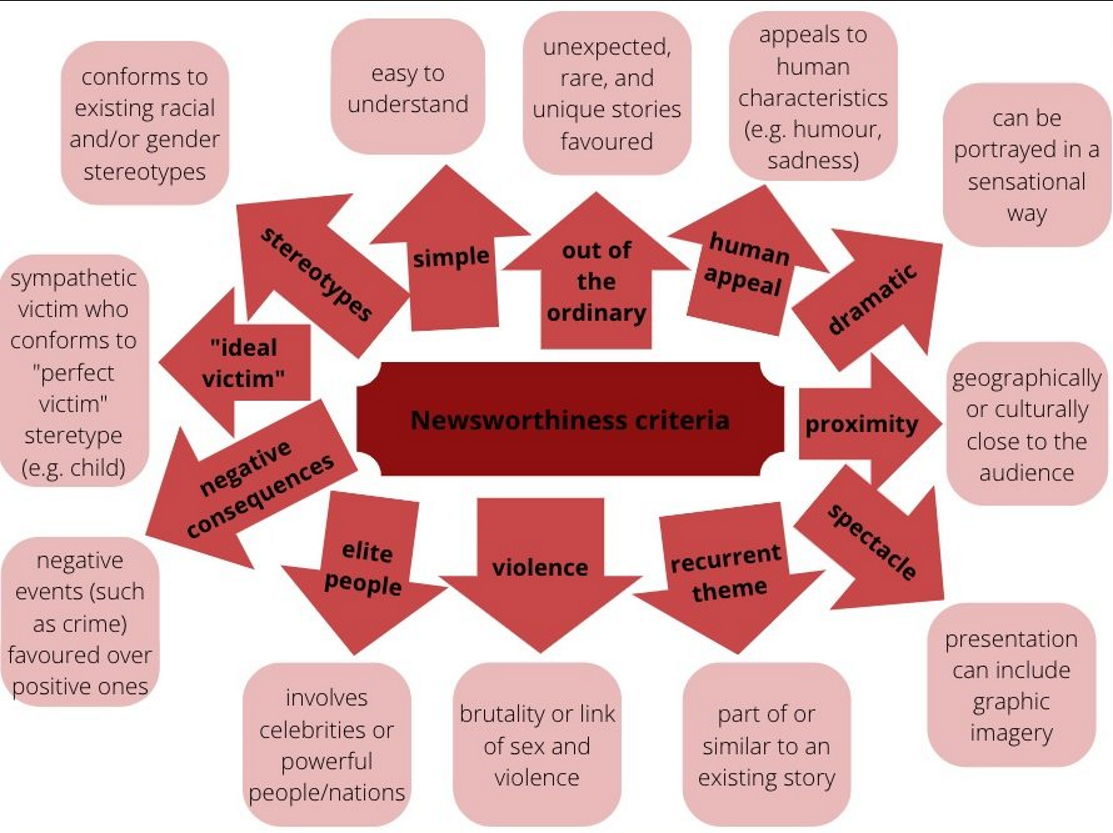
\includegraphics[width = 4in]{Newsworthy.png}
    \end{center}
    \caption{Newsworthiness criteria \cite{ref: Newsworthiness Criteria Image}}
    \label{Newsworthy}
\end{figure}

\subsection{Theoretical Perspectives on the Relationship Between Crime, Media and the Public}

Due to obvious reasons, the media cannot show the whole picture. Hence the question arises, who decides which stories to tell and how to tell them?

There are several models which discuss which story to show or are shown.

\begin{itemize}
    \item Market Model: Media is a business and crime news is a product that meets market. There is no need to regulate the market.
    
    \item Social Responsibility Model: Media is a tool for developing an informed citizenry and media requires regulation.
    
    \item Propaganda Model: Media contents represent the itnerests of the powerful and street crimes serves to divert attention.
    
    \item Organizational Model: Content of news is dictated by the routines of news production and reliance on established sources and story lines.
    
    \item Cultural Studies Model: Media content is a cultural product that serves to socially construct meaning and media representation may produce and reproduce social constructions and may be contested
\end{itemize}

\subsection{How Media Frame Portrayals of Offenders, Victims, and Police}

Frame sets limits of what you can see, similar thing happen to media framing. It is done using images, positioning of the content on the news paper and using stylised, bold/italic fonts.

The rarest crimes receive the most coverage, while the most common crimes rarely receive coverage. \textbf{Racialisation of crime} is also prevelant, that is people from vlnurable (racial, castist or female) are blamed for being both victim and offender. Media also tend to portray gangs as highly organised. Views which differ from enforcements have hard time to get coverage in the media.

New media shift the role of the audience from passive consumers to active participants. Looping” between the legacy and new media is apparent. Looping refers to the recycling of media content in different formats, different contexts, and different outlets.

\section{Race and Crime}

\subsection{The Origins of Race and Racism}

Race is a social invention, also referred to as a social construct that is, in part, a historical product of Western European colonization and the systems of Trans-Atlantic slavery.
A critical perspective on race is that, race is artificial social construct and not a natural category.

\subsection{Colonialism and Criminal Justice}

\textbf{Colonialism} often refers to how European expansionism moved throughout the world beginning in the 15th century. And with the introduction of European logic, science, rule of law, government, trade and religion, the locals are termed as savages. Colonization is the implementation of a political, legal, and economic system that is controlled through a foreign sovereign authority.

Europeans also follow \textbf{Doctrine of Discovery}, that is god has given right to conquer and colonize lands earlier inhibited by christins.

\subsection{The Practices of Race in Colonialism}

Scholars argue that colonialism is a system of governance that relies upon institutional forms of racism that develop over three stages

\begin{itemize}
    \item First, invent disctinction to separate themselves between the population to be controlled
    
    \item Second, try to justify control by using idea that colonised people are different type of humans
    
    \item Thirdly, understand yourselves as superiors
\end{itemize}

This results in \textit{kill the Indian in him, and save the man}. Today, the race as an action is an act that is “done” to someone in that people or subjects can be “racialised” by a person, an act, or a system.

\subsection{Police Racial Profiling}

Racial profiling is the use of race by police and border security to select subjects for surveillance, detention, and/or arrest. A common problem with studies of racial profiling is that the research seldom differentiates between different racial minorities.

\subsection{Intersectionality}

Intersectionality is an analytical framework for understanding how a person's various social and political identities combine to create different modes of discrimination and privilege. Intersectionality identifies multiple factors of advantage and disadvantage. Practise of racism can be divided into three categories on the bases if how they are deployed in real practice:

\begin{itemize}
    \item Overt Racism: It is kind of racism individuals experience as direct interpersonal experiences.
    
    \item Institutional Racism: Racism without racists.
    
    \item Systemic Racism: Bias or difference experienced as an 
    effect of the of social structures.
\end{itemize}

\section{Methods and Counting Crime}

\subsection{The Research Process}

An understanding of quality research methods is fundamental to informed citizenship, scientific advancement, economic activity and government decision-making. This is true for criminology also. The research process is consists of 9 steps:

\begin{enumerate}
    \item Planning
    \item Conceptualization
    \item Choice of Method
    \item Operationalization
    \item Sampling
    \item Data Collection
    \item Data Planning
    \item Analysis
    \item Application
\end{enumerate}

Most Western researchers follow the Newtonian epistemology that “scientific knowledge has to provide an objective representation of the external world,”. This ignores the connection between factors. One method more suited to criminology while data collection is talking circle in which all members of the group sit in the circle, one has a stone, only he can speak, he will pass after his talk is finished.

\subsection{Use of Research Findings}

Harm can come from how results are shared with others. For instance, if a researcher states that there are higher rates of financial exploitation in a certain Indigenous community than in the broader society, this implies that the tribal people tend to be more criminal, creating a negative stereotype. This kind of ill conclusions can cause a great harm to section of people since crime are involved.

\section{Biological Influences on Criminal Behaviour}

Biological theories allow criminologists to differentiate between the effects of environment, lived experiences, and genotype on antisocial behaviour and understand how the two interact to evaluate the impact of stress on the epigenome.In the past, many people started believing that all behaviour was based on biological traits with no room for environmental impact.

Phrenology, a theory of human behavior based upon the belief that an individual’s character and mental faculties correlate with the shape of their head, was one of the earliest biological theories of crime and laid the foundation for the development of the biological school of criminology. Franz Gall was one of the early proponents of phrenology. Biological positivism and determinism was also prevelant. All of this along with eugenics specially negative eugenics and pseudoscience led to holocaust.

\subsection{Genetics}

A common misconception is that  the link between biology and crime is primarily genetic. Most behaviours are not criminogenic on their own, but under the right circumstances could lead to a person offending. Eg, impulsivity.As with all studies of genetics, twins offer a great opportunity to study the effect of genetics on crime. Although, adoption gives a better way to study the effect of genetics in criminology as adoption provides the same environment but different genetic composition.

Person with certain genetic backgrounds are more sensitive to specific environmental triggers than others. Someone without a predisposition for criminal behaviour may never offend, irrespective of an adverse environment, and a person with a predisposition for criminal behaviour may never offend if they do not experience adversity.

The genome of person great number of genes, which may or may not be expressed and can also be in varying amounts. This is called epigenetics. Epigenetic studies help us understand why atrocities such as residential schools not only had major and long-lasting impacts on the Indigenous children who were abused, but also how the effect of this abuse is magnified as it is perpetuated biologically through the next generations.

\subsection{Brain Chemistry}

Brain has many neurotransmitters whose concentration affect our  behaviour and their concentration is affected by both genome and environment. Few neurotransmitters like serotonin, dopamine and monoamine oxidase (MAO) has significant impact on functioning of brain and hence are abused as drugs by many.

\subsection{Brain Damage and Disorders}
The frontal lobe, found from the forehead region above the eyes to the midway of the skull, is heavily involved in inhibiting inappropriate behaviour, aggression and impulsivity. This area is at the front of the head, so it is more likely to be injured in an accident or assault. Patients lose their social graces, self-control, and patience and may experience personality changes, develop anxiety or depression, demand instant gratification, or have poor planning skills. With a weak skull, children are highly susceptible to frontal brain damage.

Disease and toxins also cause damage to the brain, for example, stroke, brain tumours, meningitis, alcoholism, and cannabis. A patient with a tumour had developed a habit of sexual assault, which was stopped after the tumour was removed, but the habit returned along with the return of the tumour.

\subsection{Nutrition and Alcohol}

Neurotransmitters come from diet. Supplementary diets have shown to have massive improvements in behaviour. Foetal Alcohol Syndrome (FAS), which occurs due to prenatal alcohol consumption have serious effects on the developing brain of foetus. This result in children developing cognition, attention, communication, and perceptual deficits; hyperactivity; an inability to understand consequences; and poor peer relationships.

\section{Psychological Theories of Crime}

Psychology aims to answer the question, "Why do people break the law?". This is done via both individual approach and social approach. 


Research on children has shown that behaviour/temperament developed in the first three years of life is carried forward in the life. For a criminal those are high sensation seeking  combined with low self-control and negative emotionality combined with callous emotional trait. One of the most famous personality type classification is Myers-Brigg:
\begin{itemize}
    \item E/I: Extraversion or Introversion
    \item S/N: Sensing or Thinking
    \item T/F: Thinking or Feeling
    \item J/P: Judging or Perceiving
\end{itemize}

\subsubsection*{Nurture}

Argues that personality develops in response to childhood experiences. Freud proposed five stages of psychosexual development. According to him, human is sexual being and sexualness is expressed in different ways on different age. Erik Erikson expanded this theory throughout life span. At each stage of life, individuals face developmental challenges on the road to self-actualisation. Theories proposed by Baumrind (parenting style),Patterson (coercion theory) and Bowlby (attachment theory) use parenting style to describe behavior of children.

\subsection{Cognitive \& Cognitive-Behavioural Theories of Criminal Behaviour}

These look for faults in cognitive processes, mental development and/or a defective moral compass. These look at the way thoughts and feelings influence human behaviour. 	• The cognitive aspect of cognitive-behavioural psychology examines how reinforcement and punishment turn into thoughts, beliefs, and attitudes that maintain and justify behaviour. Bonta and Andrews (2017) summarise key links between antisocial attitudes and antisocial behaviour.

Heuristics are mental shortcuts that allow us to filter and process the massive amount of information we are faced with on a daily basis. They are necessary to make decisions but they are affected by cognitive bias.
\begin{itemize}
    \item Confirmation bias: Tendency to over-value evidence that confirms our beliefs over evidence that counters our belief
	
    \item In-group bias: Tendency to trust peers and colleagues more than those outside your group
\end{itemize}

\subsection{Medical Model of Psychology and Criminal Behaviour}

Mental illness would seem to fall solidly in the camp of individual psychology, the interface between mental illness and criminality is as much socially determined as it is individually determined. There are few "illnesses" which result in criminological behavior
\begin{itemize}
    \item Antisocial Personality Disorder: persistent, longstanding, maladaptive ways of thinking and feeling about oneself and others that detrimentally affect how one functions. Strongly linked with violence.
    
    \item Psychopathy: Interpersonal and emotional traits, such as manipulation, grandiosity and impaired empathy. Antisocial behaviour and lifestyle traits, such as impulsive behaviour sensation seeking and a parasitic lifestyle.
    
    \item Psychosis: Psychosis is a condition that impacts how your brain processes information and is present in some severe mental illnesses, including schizophrenia and mood disorders such as depression and bipolar disorder.
    
    \item  Substance Abuse Disorder: Characterised by difficulties reducing substance use. It has three part (Tripartite concept model by Goldstein), systemic crime, economically compulsive crimes and psychopharmacologically-driven crime. Delegalizing them involves increasing profit and thereby risk taking abilities of suppliers including violence. A notable example is of Portugal's war on drugs
\end{itemize}

\subsection{Trauma-Informed Neurobiology and Criminal Behaviour}
\subsubsection*{Adverse Childhood Experiences(ACE)}

ACEs have been linked to cause of death. Toxic Stress is prolonged activation of stress response systems in the absence of protective relationships. 	• Toxic stress causes the amygdala to get inflamed and hippocampus to lose volume. The individual experiences poor impulse control, challenges with deciphering when real danger is truly present, and a quickly activated fight/flight stress response system. However, this mechanism is not useful in daily life. Children facing domestic abuse in young age gets his sympathetic nervous system triggered too often.

\subsubsection*{Trauma-Informed Models of Addiction}

The trauma-informed model of addiction acknowledges a physiological, brain-based vulnerability to addiction that is influenced by genetics but also heavily impacted by supports and positive or negative experiences/influences in one’s life.

Post-traumatic stress disorder (PTSD) is caused by traumatic life events, resulting in persistent re-experiencing of the event; avoidance of feelings, thoughts, conversations or places associated with the trauma; adverse alterations in cognition and mood; and hyper-arousal. PTSD is assiciated with substance abuse.

\subsection{Evolutionary Psychology}

Evolutionary psychology posits that the ultimate function of all biological organisms is to increase their reproductive success. It looks at unconscious psychological mechanisms that would've been adaptive in the environment in which they evolved. Social mores change much more rapidly than genomes. It explains why age-crime curves aligns with sexual maturity curve

\subsection{Cultural Psychology}

It look at how individual behaviour is constructed by society. Subcultures can create norms that contradicts those of the society in which one lives in. Tough on crime policies are less effective than intervention, prevention and rehab approach.

Restorative Justice: theory of justice that focuses on the harm caused by crime and wrongdoing to people, relationships and community. It provides a framework for addressing and preventing harm that moves beyond punishment towards healing. There is need for public ceremonies or recognition of rehab. Conviction and incarceration are often highly public acts while rehab is completely private process

\subsection{Integrative Models of Criminality}
4 Models that integrate theories from individual, evolutionary and cultural approaches

\begin{itemize}
    \item Moffitt’s Developmental Taxonomy: explains the development of antisocial behaviour as affected by biology, socialisation, and stages of development. 
    \item General Aggression Model: explains the biological, personality, cognitive and social learning factors influencing an aggressive act. 
    \item Risk Needs Responsivity Model: provides a method for offender assessment and treatment by examining the needs underlying criminal behaviour. 
    \item Trauma-informed Systems of Care: combines the neurobiology of trauma with an analysis of the trauma-inducing aspects of the criminal justice system.
\end{itemize}

\section{Sociological Theories of Crime}

Sociological theories of crime help us understand why some drug use is stigmatised while other use is not, why crime is over- and under-represented across social groups, and what alternatives may exist to the individualistic punishment models that have dominated the criminal justice system since the 19th century.

\subsection{Crime and Social Norms}

It is society that determines what is criminal, not our biology or some universal moral standard. While crime is normal, it is not desirable; it is normal because it establishes the moral boundaries of a community. These lead to development of norms. 

\textbf{Anomie}: a lack of social or moral standards

\subsection{The Chicago School}

The Chicago School had a distinctly macro-level ecological approach to studying crime. Certain zones were marked by greater degrees of social disorganisation due to the transitional nature of these areas as new immigrant communities moved in and older ones moved out. Therefore, fast changing demographics is major invitation for crime. Thrasher argues that gangs are located in interstitial areas of the city, the zones between the settled, more organised neighbourhoods. Zones of transition are characterised by higher levels of residential mobility, ethnic heterogeneity, and lower socio-economic status.

\subsection{Strain Theory}

For Merton, anomie is a condition whereby society exerts pressure on the individual to achieve culturally defined goals but does not provide the institutional means to achieve them or devalues the institutional rules in favour of achieving the goals. Merton lays out five "adaptations" or "modes of adjustment" that people use to relate culturally defined goals with institutional rules. This model was specific to NA but as capitalism has spread across the world, the applicability of this model also. Ends justify the means. This theory is less useful for non-utilitarian crime such as breaking windows, spray painting walls with graffiti and shoplifting of small items.

\subsection{Delinquency as a Subculture}

It is developed by Albert Cohen. It tries to explain crimes that are non-utilitarian, malicious and negativistic. Working class are youth are taught democratic value that everyone can become rich but middle class youths achieve recognition for behaving correctly. There is inversion of values:

\begin{itemize}
    \item middle class places value on controlling aggression and respecting property
    \item the culture of the gang legitimates violence and group stealing
\end{itemize}

When theory was proposed, the status of females was closely tied to males in the 1950s, hence, Cohen argues that most female delinquency tends to be “sexual delinquency”. It fails to explain middle class gangs.

\subsection{Social Control Theory}

Developed by Travis Hirschi (1969). He asked, “Why don’t people engage in criminal behaviour in the first place?”. For him, a person's behaviour is controlled by four types of bonds which are attachment, commitment, involvement and belief. It has mixed results.

\subsection{Labelling Theory}

Roots of theory lies in new way of studying social reality known as symbolic interactionism by George Mead. He explains that we construct our social world and our sense of self through the symbols we exchange. Labelling theory was formulated by Howard Becker. In earlier formulation of labelling theory refers to the process wherein a stigmatising a label leads to a person thinking himself as a criminal.

“Social groups create deviance by making the rules whose infraction constitutes deviance, and by applying those rules to particular people and labelling them as outsiders”

\section{Learning Theories}

\subsection{Criminology and Colonialism}

Indigenous peoples have their own ways of responding to wrongdoing. Criminalisation and over-incarceration perpetuate colonial control and maintain the oppression of the Indigenous other.	The main social influences impacting Indigenous peoples’ justice involvement are structural racism, colonialism, and the Canadian state’s complicity in continued suffering.

\subsection{Learning Theories and Crime}

The social nature of our day-to-day lives has direct implications for our understanding of antisocial behaviour. Learning perspectives of crime suggest that we also learn the motivations, rationalizations, and skills of crime, substance use, and other deviant behaviour.

\subsection{Differential Association Theory}

This theory was proposed by Sutherland. Sutherland articulated the following 9 proposals

\begin{enumerate}
    \item Criminal behaviour is learned.
    \item Criminal behaviour is learned in interaction with other persons in process of communication.
    \item The principal part of the learning of criminal behaviour occurs within intimate personal groups. The important and key people in your social life are where such learning processes occur.
    \item When criminal behaviour is learned, the learning includes (a) techniques of committing the crime, which are sometimes very complicated, sometimes very simple; (b) the specific direction of motives, drives, rationalizations, and attitudes.
    \item The specific direction of motives and drives is learned from definitions of the legal codes as favourable or unfavourable
    \item A person becomes delinquent because of an excess of definitions favourable to violation of law over definitions unfavourable to violation of law.
    \item Differential associations may vary in frequency, duration, priority, and intensity.
    \item The process of learning criminal behaviour by association with criminal and anti-criminal patterns involves all of the mechanisms that are involved in any other learning.
    \item While criminal behaviour is an expression of general needs and values, it is not explained by those general needs and values, since non-criminal behaviour is an expression of the same needs and values.
\end{enumerate}

The primary component of the theory is the role of differential association(s). Individuals have a vast array of social contacts and “intimate personal groups” with whom they interact.

\subsection{Social Learning Theory}
By Burgess and Akers. It has four main components:

\begin{enumerate}
    \item Differential association
    \item Definitions
    \item Differential reinforcements
    \item Imitation
\end{enumerate}

First two components are similar to differential association theory. There are 4 types of reinforcements, positive reinceforcement, positive punishment, negative reinceforcement and negative punishment.

\subsection{Research in Learning Theories}

A meta-analysis, which synthesises all available research on a particular topic and provides an overall estimate of the empirical relationship, conducted by Pratt et al. (2010) indicated that the impact of deviant associations was moderately strong and equally as important as key factors identified by other criminological theories (i.e., self-control). Differential reinforcement had the overall weakest effects in explaining crime.

\begin{figure}
    \begin{center}
        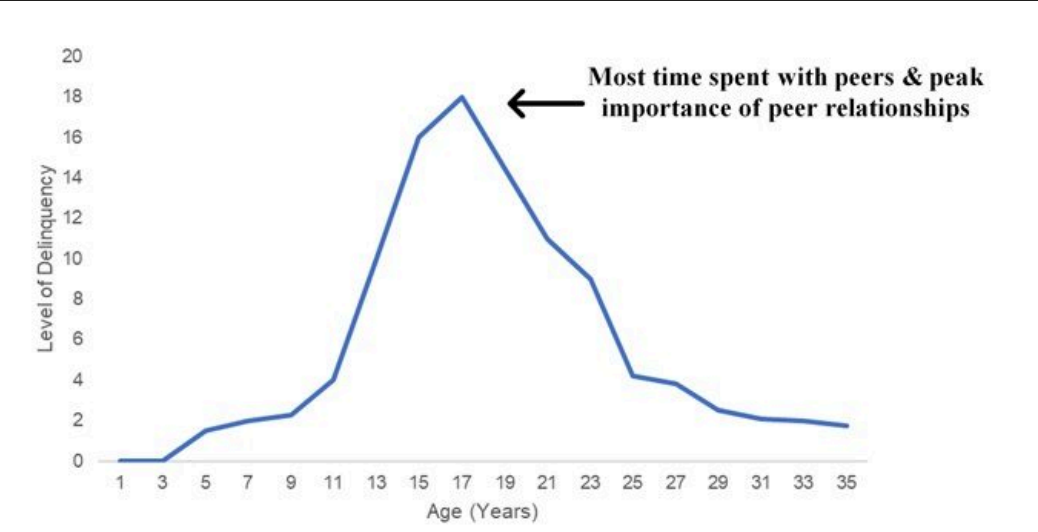
\includegraphics[width = 4in]{Age_Crime.png}
    \end{center}
    \caption{Close relationship between age and crime}
    \label{AgeCrime}
\end{figure}

\begin{itemize}
    \item Age \& Peer: Best known fact in criminology is relationship between age and crime. See image\ref{AgeCrime}
    
    \item Gender \& Peers: Research has suggested that males are exposed to deviant peers more than females. Females spend more time with parents.
    
    \item Turning Points \& Peers: find jobs, get married and possibly serve in the military. The peers at work place disapprove of the crime
\end{itemize}

\subsection{Moving Past a Monolithic Approach to Learning Theory}

Learning theories are often operationalized within western research methodologies. Learning theories do not question the role of the state or include reference to state culpability for human rights violations.

\subsection{A New Approach to Learning Theory}

Peers, friends, romantic partners, and coworkers all have the capacity to inform our attitudes towards deviance and even teach us to commit crime. Learning theories suggest that definitions acquired through associations are important. A potential weakness of social learning theories is the assumption of the universality of mechanisms attached to learning. 

\section{Critical Criminology}

Critical criminology encompasses a set of concepts and ideas examining how crime and criminal justice agencies are used as a form of social power that benefits some groups over others. Exact definition is difficult to write. Critical criminology is a form of criminology that uses a conflict perspective to question the processes, practices, and assumptions of mainstream criminology and to highlight injustice and inequality in the definition, enforcement, and response to crime. It is highly influenced by Marx and Foucault.

\subsection{The Rise of Critical Criminology}

Critical criminology initially evolved alongside criminological theories loosely called “new deviancy” that proposed new theories of crime such as labelling theory, social reaction theory, transnationalism, and interactionism, and was a significant part of a general move in the social sciences away from the dominant positivistic paradigm of criminology. Traditional criminology had effect of controlling lower classes, critical criminology tries to correct this. 	• It focuses on big picture or social structures instead of individual behaviour.

\subsection{Marx and the Basis of Critical Criminology}

\subsubsection*{Marx and the Critique of Capital}

Marx rejected the idea that societies operate based on consensus. Instead, he suggests that societies are full of conflict, which is often reflected in, and stems from, its relations of production. In chapter 26 on the secret of so-called primitive accumulation, Marx argues there is nothing natural about the creation of private property; it is only possible with state apperatus. Marx (2004) writes about bloody legislation, a swath of laws passed by the state apparatus in the 18th and 19th centuries in the Commonwealth countries that do two things:

\begin{itemize}
    \item First, they enable the creation of private property, enabling the privatisation of wealth, value, resources, land, thereby creating a powerful capitalist class.
    \item Secondly, they are used against the working class and against the lumpenproletariat who cannot work or choose not to work.
\end{itemize}

\subsubsection*{Using Marx}

William Chambliss (1964), drew on Marx’s ideas to analyse the origin of vagrancy laws (some enacted as early as 1349) and concluded that these laws were created to force people to work in factories and other places, by criminalising those who did not. The repressive state apperatus consists of military, police, judiciary and prison system bodies created for legalised violence. An instrumental Marxist position continues the understanding put forward by Marx, that the state apparatus and criminal law exists as a direct result of capitalism to uphold capitalism and the capitalist mode of production. 

A structuralist Marxist position argues that governments are somewhat autonomous and are not simply installed by the owning class. Structuralists offer a compelling set of arguments about the law-society relationship. This includes how ideas of human rights and democracy become used to justify and legitimate oppressive law. Police rarely enforce laws against white collar crime and they are difficult to govern also.

\subsection{Post-Structuralism: Foucault and Critical Criminology}

\subsubsection*{Foucault, Marx and Power}

Foucault views power via language and how we think and know about things, or in other words, how power works between people, not on people. What makes Foucault’s work important is that he extends or broadens the analysis of power away from economic re/oppression into thinking about power existing flowing/circulating between people and groups/institutions. There are three phases of his work

\begin{enumerate}
    \item Archaeological phase: emergence of discourse, power is not thought as repressive but is based on knowledge. Law as a discourse or a mechanism for categorising people
    \item Genealogical phase: how these type of classifications or discourses turn into different, mechanism of discipline and normalisation. All institutions like prison, school, factories make time-table to bring discipline.
    \item Phase of ethics: self-control or self-discipline and ultimately to how individuals engage in “care of the self” or makes themselves up as people or what he called an “ethical self. Foucault is careful to note that self-governance does not happen in a vacuum.
\end{enumerate}

Foucault, equating power with law and the state creates a sterilising political consequence meaning that it stops any other way of thinking about law except as oppressive. His work has led to new area of work called governmentality studies.

\subsubsection*{Garland, Governmentality and the Culture of Control}

David Garland picked up on Foucault’s concept of governmentality and his method of genealogy or history of the present. He was interested in penal welfare state, government programs that focus on helping criminal offenders to stop offending by providing treatment or to provide for the welfare of prisoners. He details how the system moved from a system of punishment and rehabilitative justice (where those convicted of crimes received treatment for what caused their offending) to one of safety and risk management (the management of spaces and people who were risky). This creates new culture of crime control focused on three things:

\begin{itemize}
    \item The transformation of penal welfarism/rehabilitative punishment
    \item A criminology of control
    \item One that uses economic style of reasoning
\end{itemize}

Garland outlines how rehabilitation gets redefined away from the offender’s needs to the safety of the victim and protection of society. For the criminal justice system, he argues that new culture of crime control changes the way we think about people who break the law; we begin to see them not as people who need rehabilitation, but as others that pose risk and as delinquents to be feared, controlled, and responsibilised.

\subsection{Emergent Elements of Critical Criminology}

\subsubsection*{Police and Penal Abolition}

Prison abolition, sometimes called penal abolition, focuses on the whole set of sanctions, rules and punishments involved in institutional and community corrections. However, the idea of police abolition has recently become more popular. 

McDowell’s (2019) article on insurgent safety theorises alternatives to policing and argues that state-sponsored social control fails to provide real safety against harm/transgression and fails to reduce it. They argue that community-based safety is the only way to reduce harm/transgression and achieve safety.

Nicolas Carrier has written about the blind spots of .abolitionist thinking, and the need for penal abolitionists to think seriously about the kinds of limit cases or the most difficult cases for abolitionists to address. These would include mass murderers or offenders who hurt children.

\subsubsection*{Convict Criminology}

Convict criminology is an approach to criminology that privileges the voices and standpoints of persons who have been criminalised or who have been affected by the criminal justice system (Richards \& Ross, 2001). The works of convict criminology are experiential and provide insights from inside prisons and jails, which is important because scholarly criminological work that is more or less based on deductive academic concepts can not only be wrong, but also be harmful and alienating to people who have experienced the harms of the criminal justice system.

\subsubsection*{New Research Tools for Critical Criminology}

Many methods of critical criminology are anti-positivist in orientation. New methods used to study without the cloud created by agencies itself include FOI requests and the use of computational methods. FOI (Freedom Of Information) requests: a tool to use in social science research to investigate state and criminal justice practices that accesses state records that would not otherwise be disclosed. More critical criminologists are turning to FOI requests as a form of qualitative research to investigate state and criminal justice practices. FOI requests allow access to state records that would otherwise not be disclosed (Walby \& Luscombe, 2017, 2019). FOI is similar to the RTI.

Computational social science involves using computers to model, simulate and analyse social phenomena, and to assess patterns and trends in working with big data. It includes sentiment analysis and social media sentiment analysis (SMSA) to know what people are thinking. By using computers for SMSA, the results are quite accurate for large sample altough for single response the computer may lack resourse to identify sarcasm and heavy words.

\section{Feminist Criminology}

Gender still plays in the criminal justice system, both in the victimisation and criminalisation of women, and the presence of sexism and racism in criminology at large (Chesney-Lind, 2020). Chesney-Lind has been referred to as the "mother of feminist criminology." Many have tried to shift focus of feminist criminology away from the white, middle-class, heterosexual women.

\subsection{Foundations of Feminist Criminology}

Primarily, feminism argues that women suffer discrimination because they belong to a particular sex category (female) or gender (woman), and that women’s needs are denied or ignored because of their sex. There are many types of feminism, namely

\begin{itemize}
    \item \textbf{Liberal Feminism}: Believes is equal society with abolition of discriminatory practices. Drawback is that they ignore that women's needs and risk factors differ from men
    \item \textbf{Radical Feminism}: Views the existing social structure as patriarchal and structured in a way to keep control over women
    \item \textbf{Marxist Feminism}: They also believe society to be oppressive against women and forces them to do only low paying jobs.
    \item \textbf{Socialist Feminism}: Combination of radical and Marxist theory.Socialist feminists argue these differences in power and class can account for gendered differences in offending – particularly in how men commit more violent crime than women (Winterdyk, 2020).
    \item \textbf{Post-Modern Feminism}: postmodern feminism focuses on the construction of knowledge. It believe that the diversity of women needs to be highlighted when one considers how gender, crime and deviance intersects to inform reality (Ugwudike, 2015, p. 157).
    \item \textbf{Intersectional Feminism}: Winterdyk (2020) notes that some academics add a sixth perspective. Intersectional feminists address the failure of the above perspectives to consider how gender intersects with other inequalities, including race, class, ethnicity, ability, gender identities, and sexual orientation
\end{itemize}

There are few four waves in feminisim. First one was for suffrage in the 1900s, second one was for gender equality and attention to a wide variety of issues directly and disproportionately affecting women, including domestic violence and intimate partner violence [IPV] employment discrimination, and reproductive rights in the 1950s. This is wave when Feminist criminology was started.

Third wave (1990s) focused on diverse and varied experiences of discrimination and sexism, including the ways in which aspects such as race, class, income, and education impacted such experiences. It also brought intersectionality forward. The last and ongoing wave is characterized by online tools and \#MeToo is a significant part of it.

\subsection{Critiques of Existing Criminological Theory}

Feminist criminologists recognised that theories of crime and deviance regarding women’s offending tended to take one of three paths:

\begin{itemize}
    \item Theories were openly misogynistic, negatively portraying women or situating them as “less than” men
    \item Theories were gender blind and completely ignored gender
    \item Theories took an “add women and stir” approach, meaning that the theory was primarily about men and assumed explanations for crime and deviance could be applied to women without question.
\end{itemize}

Theory of Cesare Lombroso who is known as father of criminology is openly misogynistic. For him, the criminal women were born with masculine characters or developed them. Cloward and Ohlin (followers of third path) viewed boys as having “legitimate concerns” around money and status, while girls were seen as experiencing “frivolous concerns” related to finding romantic partners .

\subsection{Issues that Brought Feminist Criminology to the Surface}

\subsubsection*{Victimisation}

Gender-based-violence is disproportionately experienced by women, whose problems are rooted in patriarchal beliefs, such as colonialism, neoliberalism and capitalism. As usual, intersectional people face greater risk of facing violence.

\subsubsection*{Sexualised Violence}

The majority victims of sexualised violence are women, especially young women of age 12-17 comprising 1/3 and 18-24 comprising 21\%. Men are perpetrators of sexual assault in 98\% cases. Women are much more likely to be blamed for their own victimisation. Feminist criminologists acknowledge that due to systemic factors, including violence, colonialization, and inequality, women are much more likely to suffer from childhood sexual abuse than men.

\subsubsection*{Criminalisation of Women}

Criminology has focused on men as offenders and this is justified as majority of police reported crimes are performed by men. Traditional criminological theories rarely accounted for female offending with rise of female offender, several theories started to come forward such as:

\begin{itemize}
    \item \textbf{Adler and Simon}: used liberation of women to account for rise in crime rate
    \item \textbf{Hagan and colleagues' power control theory}: in patriarchal homes, boys were encouraged to take risks, in egalitarian homes, girls also have freedom and hence more opportunities to engage in deviant behaviour (This theory blames working mothers for criminal tendency in daughters)
    \item \textbf{Widom, cyclic offence theory}: violence leads to substance abuse and in turn to the more crime
\end{itemize}

\subsection{Crime Statistics on Women}

In Canada, females offender represented 1/4th in police reported crime with >35\% of them property crime and female offender in four time less likely to be charged with violent crime. From 2007 to 2017, 49\% of women accused of homicide identified as indigenous versus 28\% of men (Savage, 2019). Initially women prisoners were kept with men prisoners, the prison for women were inhabitable for bears also. Indigenous women is overly represented in federal prisoners, criminogenic needs of women prisoners Is much higher than men with high criminogenic risk factors.

\subsection{Treatment in the Criminal Justice System}

Rape culture shifts the blame to women, rather than focusing on the problem of glamorised and normalised male violence. Incarcerated women have disproportionate histories of physical and psychological trauma. This reality means that they are not necessarily incarcerated for their behaviour; instead, they are incarcerated for responses to their histories of trauma (Comack \& Balfour, 2014).

Correctional programs are also heavily based on male patients gender equality is situated within colonialism, racism, and capitalism and therefore not all women have received the same benefits, as illustrated above with the experiences of racialised and sexualised populations such as Indigenous women or transgender or bisexual women.

\subsection{Critiques of Feminist Criminology}

The main critique of feminist criminology is focues on white, cis-gender women i.e. there is lack of intersectionality approach. It also does not address existing notion of masculanity and feminism. More species inclusive approach as many have linked the violence against women and animals specially female agricultural animals.

\section{Cultural Criminology}

Culture is a foundational concept of the perspective, and cultural criminology views culture as dynamic—always shifting and evolving. Cultural criminology examines the way culture both reflects and affects crime and crime control, while also examining how certain cultural practices are criminalised. It offers a critical perspectives that examines social and economic shifts in late modernity.

\subsection{Something Old}

Dr. Steven Kihm wrote, "I concede that perhaps cultural criminology is a stew of ideas borrowed from the past, brought together with fresh seasonings and presented with new style and pizazz." Using the metaphor of recycling, Ferrell illustrated a key feature of cultural criminology: its propensity to revisit and rework older ideas and breathe new life into the study of crime and crime control. While I think this is a strength of the perspective, some find fault with this approach.

\subsection{Something Borrowed}

Cultural criminology borrows from several sociological theories of deviance. Such as 

\begin{itemize}
    \item New deviance theory
    \item Subcultural theory
    \item Labelling theory
\end{itemize}

The most important contribution to what would become cultural criminology was moral panic theory developed by Jock Young (1971) and Stanley Cohen (1972).Cultural criminology focuses on the paradox that while criminal violence is condemned by law, it is also “widely commodified, consumed and celebrated” (Ferrell et al., 2008, p. 41). While cultural criminology would likely welcome works giving critical attention to issues of colonialism and indigeneity, so far the movement has been dominated by White, Western, male criminologists (Naegler \& Salman, 2016).

\subsection{Culture and Late Modernity}

Culture is a foundational concept of this perspective. Cultural criminology takes its starting point from the assumption that culture is “the stuff of collective meaning and collective identity… Culture suggests the search for meaning” (Ferrell et al., 2008, p. 2). Key feature of cultural criminology is its commitment to critical and politically engaged research. Some criminologist refer current world as post-modernist, 

\begin{itemize}
    \item Capitalism is transformed and now focused on selling lifestyles, experiences and the image.
    \item Crime is also feared but is also highly valued as an entertaining form of public spectacle.
\end{itemize}

\subsection{Boredom and Crime}

Minor acts of vandalism and transgression a key focus of cultural criminology. Crime has been blamed on factors including under-socialisation, over-socialisation, the influence of delinquent peers, poor environment, a lack of social control, flawed biology, and abnormal psychology. Cultural criminology takes as a starting point the realisation that contemporary life in Western nations is structured by features that can lead to a condition of institutionalised boredom. Boredom may generate turmoil for an individual triggering response from the mundane to explosive.

\subsection{Crime as Pleasure}

Crime provokes a great deal of worry and anxiety, but it is also a source of great pleasure in popular culture. Cultural criminology shifts the lens to the immediate experience of crime, suffering, and punishment and attends to the often conflicting feelings associated with them. Boredom and pleasure are key concepts that cultural criminology uses to make sense of actions that appear senseless.

\subsection{The Methods of Cultural Criminology}

Many of criminology’s foundational works emerged out of an idiosyncratic, impressionistic approach to ethnographic inquiry. Ethnography is a method of field research pioneered in cultural anthropology that involves immersive and lengthy interaction with cultural groups in order to learn about their ways of life and beliefs.

\subsection{Crime Media and Popular Culture}

Video games have for decades been a source of spiralling mediated moral panic about the presumed corrosive effects of violent media on youth. Video games like Grand Theft Auto and others “exemplify the broader trend toward the commodification of violence and the marketing of transgression” (Ferrell et al., 2008, p. 139). Video games and explicit online pornography are appealing in late modern times precisely because of the longstanding historical trend toward what Norbert Elias called the civilising process. Thus, Atkinson and Rodgers (2016) argue that as life has become more sanitised, safe and generally free of the threat of everyday violence, new forms of entertainment like violent videogames have become an outlet for our repressed violent impulses.

\subsection{Critiques}

Sometimes cultural criminology has been accused of romanticism by portraying criminals and deviants as cultural heroes who are fighting back against oppression through purposeful acts of transgression and deviance (Hall \& Winlow, 2007). For cultural criminology, “violence, it seems, is never only violence. It emerges from inequalities both political and perceptual” (Ferrell et al., 2008, p. 13). 

\section{Green criminology}

Green criminology is a perspective that challenges taken-for-granted notions of crime and harm in relation to humans, other species, and the natural world.

\subsection{What is Green Criminology}

Introduced by Lynch(1990). Many issues (e.g., racism, sexism, crime, environmentalism, etc.) can be related to economic, political and class interests, and more specifically, to the ability of powerful groups to manipulate and use race, class, gender, and the environment to preserve the basis of their power.

Green criminology refers to the study of environmental crimes and harms affecting human and non‐human life, ecosystems and the biosphere. More specifically, green criminology explores and analyses: the causes, consequences and prevalence of environmental crime and harm, the responses to and prevention of environmental crime and harm by the legal system (civil, criminal, regulatory) and by nongovernmental entities and social movements, as well as the meaning and mediated representations of environmental crime and harm (p. 1).

Much of traditional criminology is anthropocentric, in contrast green criminology includes environment and animals also. Green criminology not only looks at breaches of law, but also who is breaking the law, and how the justice system responds to such breaches. Green criminology embraces a zemiological approach, which entails the study of social harm. This poses critical question, who determines what is harmful and who defines what is criminal? Many legal actions have worse impact than the regular street crime for example strip mining. According to green criminology, crime serves to maintain power relations.

\subsection{What is the Difference Between Green Criminology and Environmental Criminology?}

Environmental criminology concerns with how surrounding affect the crime and what changes to be done to environment to reduce crime while green criminology also tries to address how changes surrounding to reduce will affect nature. Environmental criminology is also understood as traditional criminology as it consists mainly of surrounding studies in classiscal view. See Table \ref{Trad_vs_Green}

\begin{table}
    \centering
    \begin{tabular}{|p{1.5cm}|p{6cm}|p{7.5cm}|}
        \hline
        \ & Traditional Criminology & Green Criminology \\
        \hline
        Scope & Anthropocentric - Focus on humans, as perpetrators and victims & Non-speciesist – includes environment and animals, both human and non-human \\
        \hline
        View of Crime & Examines breaches of the law as the problem & Moves beyond the Criminal Code and regulatory laws, questions the role of power, and asks who is breaking the law and how the justice system responds\\
        \hline
        Harm & Narrow definition of harm – focus primarily on harms resulting from acts deemed illegal & Zemiological – study of social harms, including harms resulting from both legal and illegal actions.  Asks who determines what is harmful and what is criminal\\
        \hline
        Justice / Injustice & Crimes seen as acts committed against the state; does consider marginalization in perpetration and victimization of crime & Focus on injustices resulting from actions or inactions of corporations, governments, and individuals.  Calls attention to injustices disproportionately experienced by marginalized groups.\\
        \hline
    \end{tabular}
    \caption{Difference Betweeb Traditional and Green Criminology}
    \label{Trad_vs_Green}
\end{table}

\subsection{Ecophilosophies Within Green Criminology}

Brisman and South (2019) identify three main ecophilosophies within green criminology:

\begin{itemize}
    \item Anthropocentrism: emphasizes  moral and biological superiority of humans
    \item Ecocentrism: based on the idea that humans and their activities are inextricably interconnected with the rest of the natural world, it seeks best balance between the other two
    \item Biocentrism: perceives humans as just one more species
\end{itemize}

\subsection{Green Criminology and Victimisation}

For green criminology victim is not related to humans. Green criminology offers three distinct justice perspectives that often work in harmony to provide a comprehensive picture of green victimisation:

\begin{itemize}
    \item The environmental justice perspective
    \item The species justice perspective
    \item The ecological justice perspective.
\end{itemize}

The recent trend of the deceptive use of “green” language (or even the actual colour green in packaging) is known as \textbf{greenwashing}. That is, advertising products as being ecofriendly even when they are not. 

\subsubsection*{The Environmental Justice Perspective}

Environmental justice perspective states that environmental pollution does not harm everyone equally, people of race and intersectionality are more exposed to the environmental "bad."

\subsubsection*{The Species Justice Perspective}

A species justice perspective looks at the obligations and duties owed to non-human animals from perspectives such as a utilitarian moral calculus (maximising overall pleasure and minimising overall pain), the inherent value and rights of sentient creatures, or an ethic of welfare and responsible care. Humans have complex and, arguably, \textit{dramatically inconsistent} relationships with animals.

\subsubsection*{The Ecological Justice Perspective}

In this perspective even the mountains, lakes… are also entitled as deserving of protection and preservation. A brief comparision of threee perspectives can be seen in the Table \ref{three_perspective}

\begin{table}
    \centering
    \begin{tabular}{|p{2.5 cm}|p{12.5 cm}|}
        \hline
        Environmental Justice &  Justice as grounded in overcoming the disproportionate impact of environmental harms on marginalized groups in society (defined in terms of race, gender, class or other factors and their intersection)\\
        & Anthropocentric orientation \\
        \hline
        Species Justice & Justice as concerned with living creatures having intrinsic value and the rights, obligations and duties owed to them as a result \\
        & Biocentric orientation \\
        \hline
        Ecological Justice & Justice as recognizing that while humans inevitably impact natural entities and the natural world, they are worthy of protection in their own right and not just as resources to be exploited or used instrumentally \\
        & Ecocentric Orientation \\
        \hline
    \end{tabular}
    \caption{Comparision between the three green justice perspectives}
    \label{three_perspective}
\end{table}

\subsection{Linking Ecophilosophies, Justice Perspectives, and Indigenous Ways of Knowing}

The particular capacity of humans to “develop and deploy means of production that have global consequences means that humans have a unique responsibility to ensure that such production methods do not exceed the ecospheric limits of the planet.” Truly ecocentric approach to environmental harm should develop from the iterative interaction of environmental justice, species justice and ecological justice perspectives – through which their differences, inconsistencies and antagonisms are resolved.

\section{Victimology}

Victimology is the scientific study of victimisation within society. It is not study of victims. Victim, survivor, thriver and overcomer are different words used in victimology. Survivor word is preferred within feminist scholarship.

\subsection{Theories of Victimisation}

Quinney argued that “the victim” is a socially constructed phenomenon meaning that for someone to be recognised as a victim, there needs to be some agreement within society. Christie developed a typology for an ideal victim. Victim is perceived as weak, engaged in a respectable activity, not seen as responsible for contributing to their victimisation, and the offender is big and bad and unknown to the victim.

\subsubsection*{Victim Precipitation Theory}

Proposed by Marvin Wolfgang (1957). Victim precipitation refers to situations where the victim was the initial aggressor in the action that led to their harm or loss. In a quarter (26\%), the visctim was the first victim to engage in physical violence. Major criticism of this theory is the assumption that the victim and the offender enter into an interaction as equals, dismissing any power imbalances and/or dynamics at hand. This also lead to victim blaming. Victim blaming occurs when the victim of a crime is held responsible, in whole or in part, for their own victimisation.

\subsubsection*{Routine Activity Theory}

Cohen and Felson (1979) posited that the risk of criminal victimisation increases when there is the convergence of 

\begin{itemize}
    \item the presence of a motivated offender
    \item an availability of suitable targets
    \item a lack of capable guardianship (i.e. someone who could intervene to prevent the crime from being committed)
\end{itemize}

This theory has met some criticism in the context of victimology as it assumes that a victim can lessen the offender’s motivation by being less of a suitable target and ignorance of power play

\subsubsection*{Critical Criminology}

Critical victimology combines the concept of the ideal victim with intersectionality in an effort to deconstruct victim blaming by calling attention to the ways race, gender, class, and other identities shape social constructions of victimisation (Spencer \& Walklate, 2016).

\subsection{Measuring Victimisation}

In Canada, victimisation surveys are primarily used to help uncover crimes that have not been reported to the police, otherwise known as the dark figure of crime.

\subsubsection*{Challenges to Measuring Victimisation}

One of the biggest challenges in conducting victimisation research involves \textbf{operationalising} criminal victimisation. Another challenge victimisation surveys face is the mode of data collection. Lack of intersectionality is another obstacle in conducting research on criminal victimisation. 

Historically, sexual assault is a vastly under-reported crime. About 6\% of crimes are reported to police. The main reasons for not reporting their sexual assault victimization to the police include the crime was too minor, not worth taking the time to report, matter was personal or private, handled informally, did not want the hassle of dealing with police, not enough evidence, felt the police wouldn’t have considered the victimization important enough, did not think the offender would be convicted or adequately punished, and/or fear of retaliation.

\subsection{Victim Rights}

\subsubsection*{United Nations Declaration of Basic Principles of Justice for Victims of Crime and Abuse of Power}

In 1985, the General Assembly of the United Nations adopted the Declaration of Basic Principles of Justice for Victims of Crime and Abuse of Power. Brought forward by the World Society of Victimology, the declaration provided a blueprint for member states to develop their own national legislation on victims’ rights, recommending measures to provide access to information, participation, protection, assistance, restitution, and compensation.

\subsubsection*{Victim Restitution and Compensation}

Restitution occurs when the offender repays the victim for the financial losses they have incurred as a result of the crime. Restitution excludes pain and suffering, emotional distress, or other types of damages; these losses can only be assessed in civil court. Compensation occurs when the state pays financial compensation to victims of violent or personal crimes

\subsubsection*{Victim Impact Statement}

A victim impact statement is a written or oral statement made to the court by direct or indirect victims to discuss the impact of criminal victimization. The statement may include a description of the physical, financial, and/or emotional effects of the crime. The statement may be prepared by the victim themselves, by someone on behalf of the victim. These may or may not be used in the ruling.

\subsubsection*{Balancing the Rights of the Accused with Victim Rights}

Criminals are guaranteed the right to a fair trial, to legal counsel, and to be provided with information on the case against them while victims \textit{may receive} information \textit{upon request} and there is no legal action when the victim is not provided with information.

\subsection{Victim Assistance Services (Canada)}

Trauma can result in significant changes to both the neurological and physiological make-up of an individual. Victim-based services can be

\begin{itemize}
    \item Police-based: available to victims of all types of crime and trauma
    \item Court-based: available to victims of crime to enhance the understanding and participation of victims and witnesses in the court process
    \item Community-based: available to assist victims of family and sexual violence, regardless of whether the victim has reported the crime to the police
\end{itemize}

\subsection{Impacts of Victimisation}

Victimisation can affect people physically, emotionally, mentally, spiritually and possibly economically too as they have to give time to police and lawyer. After victimisation, survivors are suddenly forced to navigate many new and complicated realities, potentially interacting with healthcare providers, media, police, and victim service providers, all while grieving and being presented with complicated choices about how to move forward (Roebuck et al., 2020a). Throughout this time, friends and family may not know what to say and may be silent to avoid causing further distress or they might offer unhelpful advice (Brison, 2002).

\subsubsection*{Resilience, Posttraumatic Growth, and Posttraumatic Change}

While the pain of victimisation may never fully subside, many survivors find ways to move forward with their lives, navigating and negotiating their way through adversity—this is the process of resilience. Surviviors may also face PTSD and may also develop post-traumatic growth in domains such as elating to others, personal strength, spiritual change, appreciation of life, et. cetera.

\subsubsection*{Survivor Reactions to Services}

Some victims choose not to participate in services to avoid re-victimisation. 21 \% used specialised victim services when provided at no-cost to the victim.  Survey respondents often felt frustration when information was limited, inaccurate, and/or confusing. Dissatisfaction also arose when participants were forced to initiate contact themselves with a criminal justice professional as well as from receiving incorrect/inconsistent information from criminal justice professionals due to changes in staffing.

\subsubsection*{Trauma and Violence-Informed Care}

Trauma and violence-informed care (TVIC) approaches are policies and practices that recognize the connections between violence, trauma, negative health outcomes and behaviors (Government of Canada, 2018). Four key principles of TVIC are

\begin{itemize}
    \item understand trauma and violence and their impacts on peoples’ lives and behaviors
    \item create emotionally and physically safe environments
    \item foster opportunities for choice, collaboration, and connection
    \item provide a strengths-based and capacity-building approach to support client coping and resilience
\end{itemize}

\section{Crimes of the Powerful}

The image of the typical offender created through the way the criminal justice system operates, and through a reliance on official sources of crime data is of a young male, from the lower socio-economic strata, who is disproportionately likely to be Indigenous or Black. This image is in stark contrast to who is responsible for most physical and economic harm on our planet: middle-aged and older, affluent, white males holding positions of social, political, and economic power in society. These crimes are defined many times as regulatory offences, resulting in fines rather than prison times. Even if they are tagged crime, they are very less likely to be investigated.

\subsection{Crimes of the Powerful are White-Collar Crimes}

Edwin Sutherland defines white collar crime as "crime committed by a person of respectability and high social status in the course of his occupation." Government actions, not the actions of individuals acting alone, are responsible, by far, for most injury and death on the planet. The important feature of white-collar crime is that the individual is able to use their occupational position and socio-economic status to commit their offence and avoid detection.

\subsection{Corporate Crime}

Corporate crime is when an individual uses their position within an organisation to illegally benefit corporate interests, including boosting profits or market share. The financial losses corporate crime causes far exceed the losses associated with street crimes, like theft or robbery (avg. \$ 2119). 

\subsubsection*{Occupational Crime}

Most thefts against businesses involve employees, executives, or owners, in what is referred to as occupational crime. For example, cashier at Walmart stealing money.

\subsubsection*{Corporate Theft}

One of the biggest corporate criminal cases of all time—involving the loss of \$ 74 billion in shareholder money—was orchestrated by senior managers at the U.S. corporation Enron. He sold off all his stock before disaster. The disaster was happened due to including of future profits in the assets i.e. accounting frauds.

\subsubsection*{Corporate Tax Evasion}

Corporate tax evasion when corporations do not pay the taxes they legally owe to the government. It generally done by ocrporates opening its subsidiary's and offices (shell companies) in countries with lower taxes.

\subsubsection*{Corporate Violence}

While reports about murderers attract attention and outrage from the general public, breaches of safety regulations are responsible for much more injury and death than criminal homicide, consider Balasore railway accident. Guilty of corporate violence rarely go to prison.

\subsection{Financial Crimes}

Financial crimes refer to “large scale illegality that occurs in the world of finance and financial institutions,” such as banks and insurance companies, and because of the vast amount of money involved and the risk these crimes pose to the integrity of the economic system, they are placed in a separate category (Friedrichs, 2017, p. 153). These crimes include banking frauds, price-fixing, illegal monopolies, insider trading and a variety of unscrupulous behaviours.

\begin{table}[H]
    \centering
    \begin{tabular}{|p{15.5cm}|}
        \hline        
        \textbf{Insider Trading, Front Running, and Pump and Dump} \\
        Insider trading refers to “the buying or selling of a publicly-traded company’s stock by someone who has non-public, material information about that stock” that will likely affect its value. \\
        “Front running” is a variation of insider trading where stock brokers take advantage of information about imminent transactions that are likely to affect the value of stocks to enrich themselves. \\
        Pump and dump: This is a scheme designed to boost the price of a stock through “false, misleading, or greatly exaggerated statements”\\
        \hline
    \end{tabular}
\end{table}

\subsection{Political Crime}

Political crime refers to “governmental or political party officials engaging in illegal and improper activity for personal gain”.

\subsection{State-Organised Crime}

• Chambliss (1989, p. 184) defines state-organised crime as, “acts defined by law as criminal and committed by state officials in pursuit of their job as representatives of the state.” A more recent term, “state crimes against democracy” (or SCADs for short), has been suggested by Professor Lance deHaven-Smith of Florida State University. He defines these as, “actions or inactions by government insiders intended to manipulate democratic processes and undermine popular sovereignty.”

\subsubsection*{Illegal Surveillance}

Information collected by the government included a target’s political views, medical history, the status of their intimate relationships, and details about online sexual activities. These has been used to blackmail those who are in oppose with the governments politically.

\subsubsection*{Coup d’États}

This refers to the non-democratic, and often violent, overthrow of a government, either by those already working within the government but unhappy with its leadership, or by those outside the government who view it as a threat to their interests. In the modern age, the CIA is probably the organisation most notorious for carrying out coup d’états against socialist leaders unfriendly (or perceived to be unfriendly) to U.S. governments or corporations, or those of its allies.

\subsubsection*{Illegal Wars}

According to the rules of war established after World War II, there are only two legitimate reasons for a country to invade another country: (1) in self-defence; or (2) when authorised by the UN Security Council. The U.S. invasion of Iraq in 2003 is the type of crime largely ignored by criminologists is an example of using false narraratives to justify wars.

\subsubsection*{War Profiteering}

The main economic beneficiaries of war are corporations that sell the equipment needed to fight, such as armaments and fuel, as well as food, clothing, and shelter for the troops. Many of the defence spending is hidden from public due to security reasons and hence a easy target for misuse.

\subsubsection*{Colonialism and Slavery}

Colonialism constitutes the largest program of state-organised harms in world history. Imperial conquests conducted by European states such as Spain, France, and Britain involved the enslavement of millions of Africans; the dispossession of Indigenous land; mass murder; destruction of culture, communities and families; physical, sexual, and emotional abuse; and human experimentation without informed consent. Bishop Desmond Tutu of South Africa, put it this way: “When the missionaries first came to Africa they had the Bible and we had the land. They said, ‘let us pray’. We closed our eyes. When we opened them, we had the Bible and they had the land”.

\subsection{Challenges Related to White-Collar Crimes}

Victims are not always aware of victimisation, for example, victim of price-fixing. Racial minorities are more likely to be victims. Less developed countries are at high risk for example consumer products found to be hazardous in North America may be shipped to less developed countries where a combination of lax regulatory regimes, higher rates of illiteracy, and widespread poverty means the most marginalised are at higher risk. Economic costs exceed street crimes.

There is a definite lack of research attention devoted to crimes of the powerful.Laws and regulations aimed at the crimes of the powerful are inadequate and often do not exist; if they do, they frequently result in fines or monetary payouts awarded after civil litigation. They usually do not result in prison. Revealing the crimes of the powerful can be dangerous. Powerful peoples have known to hire people to punish even with death for whom who try to raise voice against them.

\section{Environmental Criminology}

\subsubsection*{The Origins of Environmental Criminology}

In 1979, C. Ray Jeffery coined the term environmental criminology. The environment is broadly consists of 

\begin{itemize}
    \item the physical design of places (architecture)
    \item the built environment (types of buildings, roadways, land use etc.)
    \item legal and social institutions.
\end{itemize}

Environmental criminology can be also described as spatial criminology. Spatial criminology concerns the relationship between physical spaces and crime.

\subsection{A Basic Understanding of Environmental Criminology}

Those who study environmental criminology are primarily focused on the criminal event and not the individual criminal, they are interested in the spatial distribution of crime, victimisation, or offenders in society.

\subsection{Environmental Criminology and Green Criminology}

For brevity purposes, green criminology represents the branch of criminology that deals with research into criminality against the environment and associated phenomena (e.g., animal cruelty) (Fitzgerald et al., 2013; Fitzgerald et al., 2016). On the other hand, environmental criminology is a branch of criminology that deals with researching physical and social determinations of patterns of criminal behaviour and is closely connected with situational crime prevention (White, 2013).

\subsection{Routine Activity Theory}

It was first posited in 1979 by Lawrence Cohen and Marcus Felson. Routine activity theory predicts how changes in social and economic conditions influence crime and victimisation and it has become one of the most cited theories in criminology. Routine activity is “any recurrent and prevalent activities which provide for basic population and individual needs, whatever their biological or cultural origins”

Routine activity theory has traditionally been used to explain residential break and enter, burglary, domestic violence, and physical assault. Routine activity theory focuses on crimes that involve 
\begin{itemize}
    \item at minimum, one motivated offender
    \item one suitable personal or property target
    \item the absence of a guardian capable of preventing such a violation
\end{itemize}

\subsection{Geometric Theory}

The geometric theory of crime explains patterns of crime based on the geographic dimension of human activity patterns. The focus here is not on the motivation for crime, but rather the perceived opportunities for crime that exist within the urban spatial structure.

The city consists of four elements: nodes, paths, districtsand edges. Maps represents our activity space. Over time, our activity space becomes our awareness space, because “we develop knowledge and attachments to different locations such that we develop a sense of place, feeling comfortable in some areas and uncomfortable in other areas.” We manage risks by knowing such areas. Understanding how someone moves through (and becomes part of) an environment can provide an understanding of how potential offenders move through (and become part of) that same environment.

\subsection{Rational Choice Theory}

This theory was first posited in 1987 by Ronald Clarke and Derek Cornish. The fundamental concept within rational choice theory is rationality. Rationality refers to the role of reasoning in human behaviour and views crime as the outcome of an individual thinking through the possible rewards and downsides of a criminal act. Rational choice theory purports that a potential offender must make four primary choices:

\begin{itemize}
    \item whether or not to commit a crime
    \item whether or not to select a particular target
    \item how frequently to offend
    \item whether or not to desist from crime.
\end{itemize}

If a person commits a property crime, for example, this does not mean this same person will commit a sexual assault. Rational choice theory is most often used in situational crime prevention strategies as this approach seeks to modify the environment within which crime occurs. There are five operating principles using this approach:

\begin{itemize}
    \item increase the perceived effort
    \item increase the perceived risks
    \item reduce the anticipated rewards
    \item reduce provocations
    \item remove the excuses for crime
\end{itemize}

\subsection{Pattern Theory}

Pattern theory examines the ways targets come to the attention of offenders and how this influences the distribution of crime events over time and space. Pattern theory “links place with desirable targets and the context within which they are found by focusing on how places come to the attention of potential offenders”

\subsection{Applications of Environmental Criminology}

Researchers have found that offenders often commit crimes near their current and/or former residential homes, near family members  and near friends. Lastly, some researchers also found that offenders return to previously targeted areas and commit offences close to other routine activity nodes, such as their schools, workplaces, and leisure activity locations.

\subsection{The Strengths and Limitations of Environmental Criminology Theories}

\subsubsection*{Strengths}

Environmental criminology theories can help shed light on our understanding of the lived experiences of Indigenous peoples. Environmental criminology has been praised for the shift in its focus from criminals to conventional people (those who did not break the law), aiding in a better understanding of crime events and their prevention. It has also rejected the evil-causes-evil fallacy by arguing that offenders make rational choices in crime situations and are born with similar natures.

\subsubsection*{Limitations}

Environmental criminology theories can hinder our understanding of the lived experiences of Indigenous peoples. Environmental criminology theories need to develop a fuller understanding of the risk of victimisation. These theories fail to look at why some individuals are less exposed to risk. Environmental criminology theories neglect to look at the role of inequality in the broader social environment.

\section{Restorative, Transformative Justice}

\subsection{Restorative Justice: A Paradigm Shift}

Restorative justice approaches are informed by values, principles, and practices from a variety of sources including Indigenous ways of knowing, faith-based traditions, peacemaking criminology, the Victims’ Rights Movement, penal abolition, and community justice initiatives. Howard Zehr is a criminology affectionately known in the field as the “grandfather of restorative justice”.

\subsection{Justice as Healing}

Restorative justice aims to put victims’ needs at the centre of the justice process and to encourage greater community engagement through inclusive and collaborative processes. Rather than focusing on rules, restorative justice focuses on the emotional and relational dimensions of crime. Restorative processes can occur at various stages of criminal justice/legal processes. The Table \ref{criminalJ_restorativeJ} shows difference between criminal justice and restorative justice.

\begin{table}
    \centering
    \begin{tabular}{|p{7.5cm}|p{7.5cm}|}
        \hline
        \textbf{Criminal Justice} & \textbf{Restorative Justice} \\
        \hline
        Crime is a violation of the law and the state & Crime is a violation of people and relationships \\
        \hline
        Violations create guilt &  Violations create obligations \\
        \hline
        Justice requires the state to determine blame (guilt) and impose pain (punishment) or expect they get better (rehabilitation) & Justice involves victims, offenders, and community members in an effort to repair the harm, to “put things right” \\
        \hline
        Central focus: offenders getting what they deserve & Central focus: victim needs and offender and community responsibility for repairing harm and promoting accountability \\
        \hline
    \end{tabular}
    \caption{Criminal Justive vs. Restorative Justice}
    \label{criminalJ_restorativeJ}
\end{table}

\subsection{The Aims of Restorative Justice}

Rehabilitation is a guiding principle of criminal justice practice and usually involves interventions that focus on reducing the risk that perpetrators will cause harm in the future. Retribution also aims to reduce the likelihood that the offender or other would-be perpetrator will cause future harm. Rather than focusing on treatment, retribution seeks to impose a proportional amount of discomfort on an individual to create both general and specific deterrence. The positive impact restorative justice approaches offer for victims, offenders, and communities can be understood through relational theory which “recognizes not only that we live in relationships with others but also that relationship and connection with others is essential to the existence of the self”.

\subsection{Restorative \& Transformative Justice: Definitions and Conceptions}

Restorative justice is an approach to achieving justice that involves, to the extent possible, those who have a stake in a specific offense or harm to collectively identify and address harms, needs, and obligations in order to heal and put things as right as possible. Johnstone and Van Ness (2007) propose three conceptions: encounter, reparative, and transformative.

\subsubsection*{Encounter Definition}

Restorative justice is a process whereby the parties with a stake in a particular offense come together to determine collectively how to deal with the aftermath of the offense and its implications for the future.

\subsubsection*{Reparative Definition}

Reparative conceptions of restorative justice involve seeking non-punitive responses to fulfill reparation to people and relationships after a crime has occurred. Reparation can be symbolic and/or material.

\subsubsection*{Transformative Definition}

Restorative justice in its most comprehensive form is relational, transformative, democratic peacebuilding that attempts to transform communities and schools toward recognizing that people are not objects to be manipulated, but rather organic, interconnected, worthy human beings.

\subsection{Justice Stakeholders}

Restorative justice aims to meaningfully include three stakeholders in the justice process: victim, offender, and community.

\subsubsection*{Victims}

The focus of the current justice system is on apprehending, prosecuting, and sentencing people who cause harm or “offenders.” Restorative justice attempts to minimise the risk of secondary victimisation by placing victims’ needs at the centre of the justice. The promise of restorative justice is:

\begin{itemize}
    \item an elevation of the victim’s status
    \item identification of the victim as the person that the offender is first and foremost accountable to
    \item greater and more meaningful participation in the legal process,
    \item a focus on harm to provide a necessary identification of victim needs as the starting point of justice, and
    \item the creation of a space where victims in the aftermath of trauma can control the process of justice.
\end{itemize}

\subsubsection*{Offenders}

From a restorative justice perspective, harming another person creates obligations on the part of the harm-doer to take responsibility for what happened and to be accountable through making things as right as possible. Offenders are invited to take part in acts of reparation/restoration by being willing to repair both material and symbolic dimensions of harm.

\subsubsection*{Community}

From a restorative, transformative perspective, communities are obligated to play a role in both providing support to those directly impacted and holding themselves and others accountable for creating the conditions for crime and harm to occur. A community can include anyone who feels connected to the harm or the people involved in the harm. Community members—those directly or indirectly impacted by the harm.

\begin{figure}
    \begin{center}
        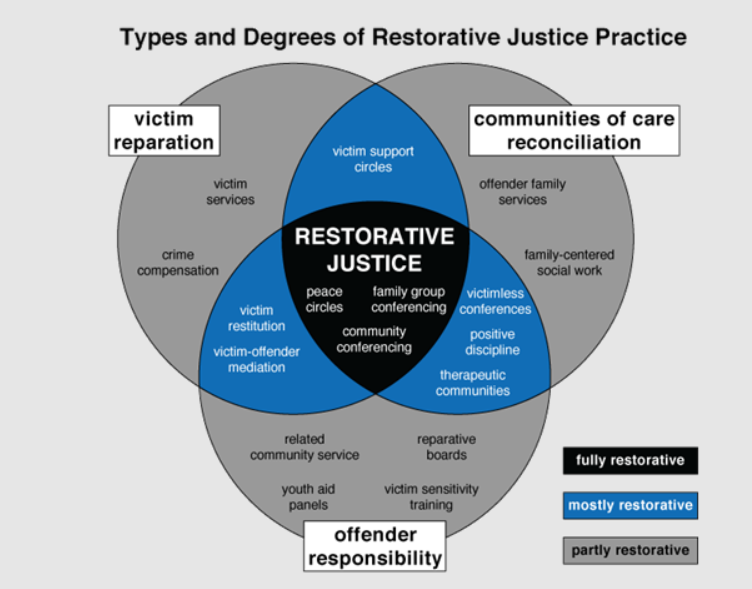
\includegraphics[width = 4in]{Restorative_Justice.png}
    \end{center}
    \caption{Types and Degrees of Restorative Justice Practices \cite{ref: Types and Degrees of Restorative Justice Practice}}
    \label{RestorativeJ}
\end{figure}

\subsection{Restorative Justice Models}

For a process to move forward, several criteria must be met. In most instances, the person who caused the harm must accept responsibility for their actions and be open to making reparation. The victim/survivor must participate voluntarily and be provided voice and choice in how the process will unfold. Community members might also be included and must be informed and prepared to ensure the process itself upholds the values of respect, honesty, accountability, and safety.

\subsubsection*{Victim-Offender Dialogue}

The approach involves facilitating communication between the victim/survivor and the person who caused them harm. The dialogue could be direct/face-to-face or indirect through exchanging letters or video recorded messages. People are not expected to leave the dialogue as friends: rather, the aims are to have gained understanding of what happened, the harm caused, and what is required for reparation to begin.

\subsubsection*{Conferencing}

These sometimes called Victim-Offender Conferencing or Family Group Conferencing. conferences are similar to victim-offender dialogue but involve more participants who can be family members and other resource people. Conferencing participants provide support to both victims and offenders, often providing accountability for the offender to complete the reparations they have agreed to.

\subsubsection*{Circles}

Peacemaking circles have deep roots in many Indigenous traditions and worldviews.  A more traditional peacemaking circle involved the entire community, leaders, Elders and respected knowledge holders to resolve an issue. These circle processes are convened to reintegrate people into the community following crime or incarceration or used instead of the formal court process.

\subsection{Restorative Justice \& Indigenous Ways of Knowing}

There are important features that make Indigenous legal traditions quite different from restorative justice processes, including how Indigenous legal traditions often use proactive/preventative strategies mediated through kinship networks. Decolonisation requires decolonising our minds and our imagination—a rethinking of possibilities.

\subsection{Benefits \& Critiques of Restorative Justice}

\subsubsection*{Benefits}

For victimes/survirvors, it offers direct accountability from the person who caused harm, opportunities to be heard and understood, increased satisfaction with justice. For offenders, it offers opportunities to start to make things right and be accountable, opportunities for meaningful direct or indirect communication (exchange of letters, messages, videos, etc.) with others involved in the harm. For the community it offers increased sense of safety, reduced re-offending and strengthening the sense of community and  building relationships through participation in justice

\subsubsection*{Critiques}

Transformative approaches reject punishment and retribution as primary goals, some people perceive that it is “soft on crime.” Criminal justice stakeholders trained in and conditioned to the punitive system may resist adopting new practices and practicality of shifting an entire criminal justice system to a new paradigm. Lacking established and universally agreed-upon standards of practice, participants may experience inconsistent processes in different jurisdictions and facilitators with varying levels of expertise, which may cause harm or lessen faith in the fairness and efficacy of the system. Because many restorative principles originate in the traditional practices of Indigenous and other cultures, there is a risk of cultural appropriation and disrespectful distortions that perpetuate the exploitation and oppression of marginalised peoples.

\section{Criminology in Indian Context}

\subsection{Comparative Criminology}

Every nation has a different social and legal control system and a different way of thinking about crime. This is the basis of comparative criminology. Comparative criminology is widely recognised as a cross cultural comparison of crime rates; however, it is rather a scientific approach which seeks to analyse the commonalities and differences of a given phenomenon of two or more countries.

Based upon types of laws and punishments, there are four kinds of society. Those are folk-communal society, urban-communal society, urban industrial society and bureaucratic society. Similarly. there are four different legal traditionals; common law, civil law, socialist law and religious law (e.g. Shariat Law).

\subsection{Criminology in India}

One of the oldest centre for criminology was set up in 1954 as the then erstwhile Department of Criminology and Correctional Administration (CCA) at Tata Institute of Social Sciences, Mumbai. Another significant development was the setting up of an Expert committee by the UGC to suggest steps to bring Criminolog and Forensic Science into the general stream of University education as a result of the resolutions taken at the UNESCO symposium in London, 1955. Lok Nayak Jayaprakash Narayan National Institute of Criminology and Forensic Sciences, Delhi- 1972. It became an independent department directly under the Ministry of Home Affairs in 1976.

The history of the Indian legal order shows an intricate construction of institutions and codifications which relate to the British legal system, to Hindu or Muslim traditions (partly reinvented), and, since independence, to various international interactions. Despite the urbanization, Indian society largely remains essentially rural and relationships are still rooted in religion, caste, and traditional local customs - all mechanisms of authority that can be very coercive at local level. A good example is caste system. It brings with it exploitative relationships like bonded labour or sexual harassment.

\subsection{Crime as a social problem in India}

Organised crime has significantly risen in India, so has crime against women. Large-scale organisations have also emerged for criminal activities which systematically organise the control and distribution of illicit goods and services—like drugs (narcotics), human trafficking (in India and in the Arabian countries), ransom oriented activities like kidnapping, protection money (hafta), smuggling of banned items like animal trade, artefacts etc. Criminal Procedure Code divides crimes into two heads: cognizable and non-cognizable. In the former, police is responsible to take quick action on basis of a complaint received or on receipt of credible information. Some cognizable crimes fall under the category of Indian Penal Code (IPC) while others come under the Special and Local Laws (SLL). Non-cognizable crimes, on the other hand, are supposed to be handled, pursued and managed in the Court by the affected parties

\subsubsection*{Women and Crime: Crime against Women}

“The crime rate under crimes against women was reported as 53.9 in 2015. Delhi UT has reported the highest crime rate (184.3) compared to 56.3 at all India level during the year 2015, followed by Assam (148.2), Telangana (83.1), Odisha (81.9), Rajasthan (81.5), Haryana (75.7) and West Bengal (73.4)." The NCRB (2015) document shows that the major type of crime against women is cruelty by husband or his relatives (34.6\%), followed by assault on woman with intent to outrage her modesty (25.2\%), kidnapping and abduction of women (18.1\%) and rape (10.6\%). What sets this particular crime aside is the Supreme Court‘s decision on Section 498A of IPC. This section protected married women against domestic abuse by the husband or his relatives and SC in the month of July, 2017 decided that this law was being misused.


According to the NCRB‘s 2009 report, women criminals comprise of only 6.3\% of the total criminals. Many research points their unequal treatment as cause of their criminal activity. It is also interesting to note that a number of women are misusing laws that has been formulated for their welfare against men. This is called legal terrorism in print media.

\subsubsection*{Kidnapping and Abduction}

NCRB report (2015) shows a 238.3\% increase in the incidents of kidnapping and abduction. This figure is astonishing as with increased surveillance kidnapping should have become much harder. But with the technological front serving as a backbone to crime collecting ransom money and dispatching untraceable threats has become much easier.

\subsubsection*{Robbery}

A 115.4\% increase in the crime seems ironical. For the same reason as above, one would expect the frequency of robbery to decline. But it seems that with more sophisticated technology break and entering is becoming more commonplace.

\subsection{Factors affecting crime in India}

As with general criminology factors such as poverty, reduction of gender ratio, disorganization and disintegration of family and society, individual level psychological factors like unhealthy parenting, deficient‘ parental control and non-cordial relations within family, maltreatment in childhood, domestic violence, alcoholism, drug addiction etc are affecting crime rates.

The theories aforementioned in above sections are also valid in case of India.

\subsection{Prevention of crime}

Recently it has been clearly laid down by the Supreme Court of India that the manner in which offenders are treated in jails is an extension of the judicial process itself and the rights of the prisoners are to be protected by the court. The prisons systems should also be independent of the bias of socio-political system.  Observational homes (or Remand houses) are an attempt in this very humane direction.

The study of criminology makes it evident that the causation of crime is multifaceted and loopholes in the law aren‘t the solitary reason for a crime to be committed. What has been evident to scholars and even contemporary media is that one crime doesn‘t make an individual a criminal, but the prison culture, the social tax of being a criminal and the degradation of the status quo do. 

A realisation that dawned upon the government was that the locals know more and care more about the nature and its preservation. Including locals, raising awareness and organising them into a task force of vigilance could be of great help in preventing criminal activities. In December of 2015, Ministry of Women and Child Development released an official document about the increasing rate of cybercrimes and described how the existing laws can be used to combat it.

The core of crime, criminals and rising rates of crimes can be condensed in a single sentence: "resources are limited". Social workers, politicians, administrators of law and the police force need to join hands and encourage the public to show empathy to fragment of the population that belongs to the lowest strata.

\subsection{Some Classic Case of Case Studies of Criminals in India}

There are some landmark criminal cases in India which changed the direction of criminology in India. Some of them are 

\begin{itemize}
    \item Murder of Naina Sahni – The Tandoor Case
    \item Nirbhaya Rape and Fatal Assault Case
    \item Nithari Killings
    \item Charles Sobhraj – the Bikini Killer
    \item Priyadarshini Mattoo Case
\end{itemize}

\newpage

\begin{thebibliography}{99}
    \bibitem{ref: Introduction to Criminology}
    {Introduction to Criminology\\
    \url{https://open.umn.edu/opentextbooks/textbooks/1327}}

    \bibitem{ref: Newsworthiness Criteria Image}
    {Newsworthiness Criteria\\
    \url{https://kpu.pressbooks.pub/app/uploads/sites/199/2022/08/Figure-1-red-version-e1661459196776.jpeg}}

    \bibitem{ref: Types and Degrees of Restorative Justice Practice}
    {Restorative Justice\\
    \url{https://kpu.pressbooks.pub/app/uploads/sites/199/2022/02/Picture5.png}}


\end{thebibliography}

\end{document}